\documentclass[a4paper]{article}
\usepackage[spanish]{babel}
\usepackage[utf8]{inputenc}
\usepackage{charter}   % tipografia
\usepackage{graphicx}
%\usepackage{makeidx}
\usepackage{paralist} %itemize inline

%\usepackage{float}
%\usepackage{amsmath, amsthm, amssymb}
%\usepackage{amsfonts}
%\usepackage{sectsty}
%\usepackage{charter}
%\usepackage{wrapfig}
%\usepackage{listings}
%\lstset{language=C}


\usepackage{color} % para snipets de codigo coloreados
\usepackage{fancybox}  % para el sbox de los snipets de codigo

\definecolor{litegrey}{gray}{0.94}

% \newenvironment{sidebar}{%
% 	\begin{Sbox}\begin{minipage}{.85\textwidth}}%
% 	{\end{minipage}\end{Sbox}%
% 		\begin{center}\setlength{\fboxsep}{6pt}%
% 		\shadowbox{\TheSbox}\end{center}}
% \newenvironment{warning}{%
% 	\begin{Sbox}\begin{minipage}{.85\textwidth}\sffamily\lite\small\RaggedRight}%
% 	{\end{minipage}\end{Sbox}%
% 		\begin{center}\setlength{\fboxsep}{6pt}%
% 		\colorbox{litegrey}{\TheSbox}\end{center}}

\newenvironment{codesnippet}{%
	\begin{Sbox}\begin{minipage}{\textwidth}\sffamily\small}%
	{\end{minipage}\end{Sbox}%
		\begin{center}%
		\vspace{-0.4cm}\colorbox{litegrey}{\TheSbox}\end{center}\vspace{0.3cm}}



\usepackage{fancyhdr}
\pagestyle{fancy}

%\renewcommand{\chaptermark}[1]{\markboth{#1}{}}
\renewcommand{\sectionmark}[1]{\markright{\thesection\ - #1}}

\fancyhf{}

\fancyhead[LO]{Sección \rightmark} % \thesection\ 
\fancyfoot[LO]{\small{Nombre Apellido, Nombre Apellido, Nombre Apellido}}
\fancyfoot[RO]{\thepage}
\renewcommand{\headrulewidth}{0.5pt}
\renewcommand{\footrulewidth}{0.5pt}
\setlength{\hoffset}{-0.8in}
\setlength{\textwidth}{16cm}
%\setlength{\hoffset}{-1.1cm}
%\setlength{\textwidth}{16cm}
\setlength{\headsep}{0.5cm}
\setlength{\textheight}{25cm}
\setlength{\voffset}{-0.7in}
\setlength{\headwidth}{\textwidth}
\setlength{\headheight}{13.1pt}

\renewcommand{\baselinestretch}{1.1}  % line spacing


% \setcounter{secnumdepth}{2}
\usepackage{underscore}
\usepackage{caratula}
\usepackage{url}


% ******************************************************** %
%              TEMPLATE DE INFORME ORGA2 v0.1              %
% ******************************************************** %
% ******************************************************** %
%                                                          %
% ALGUNOS PAQUETES REQUERIDOS (EN UBUNTU):                 %
% ========================================
%                                                          %
% texlive-latex-base                                       %
% texlive-latex-recommended                                %
% texlive-fonts-recommended                                %
% texlive-latex-extra?                                     %
% texlive-lang-spanish (en ubuntu 13.10)                   %
% ******************************************************** %



\begin{document}


\thispagestyle{empty}
\materia{Organización del Computador II}
\submateria{Segundo Cuatrimestre de 2014}
\titulo{Trabajo Práctico II}
\subtitulo{subtitulo del trabajo}
\integrante{Alejandro Mignanelli}{609/11}{minga_titere@hotmail.com}
\integrante{Franco Negri}{893/13}{franconegri2004@hotmail.com}
\integrante{Federico Suárez}{610/11}{elgeniofederico@gmail.com}

\maketitle
\newpage

\thispagestyle{empty}
\vfill
\begin{abstract}
En el presente trabajo se describe la problemática de procesar información de manera eficiente cuando los mismos requieren:
\begin{enumerate}
\item Transferir grandes volumenes de datos.
\item Realizar las mismas instrucciones sobre un set de datos importante.
\end{enumerate}

\end{abstract}

\thispagestyle{empty}
\vspace{3cm}
\tableofcontents
\newpage

%\normalsize
\newpage

\section{Objetivos generales}

El objetivo de este Trabajo Práctico es mostrar las variaciones en la performance que suceden al utilizar instrucciones SIMD en comparación con código C con diversos grados de optimización realizados por el compilador cuando se manejan grandes volúmenes de datos que requieren un procesamiento similar.

Para ello se realizarán distintos experimentos sobre cuatro filtros de fotos, Cropflip, Bandas, Sierpinski y Motion Blur, tanto en código assembler, que aproveche las instrucciones SSE brindadas para los procesadores de arquitectura Intel, como en código C, al que se le aplicarán los distintos flags de optimización -O0 (predeterminado), -O1, -O2 y -O3.

El primer filtro, Cropflip, se utilizará para mostrar cuanto mejora la performance al utilizar los registros XMM para transferir grandes cantidades de información.

El segundo, tercer y cuarto filtro, se centrarán en la variación de performance (en comparación al código en C) al utilizar instrucciones SIMD, no sólo para transferir grandes volúmenes de datos sino también para procesarlos en forma paralela, es decir, realizar diversos cálculos (sumas, multiplicaciones, divisiones) tanto en representación de enteros como punto flotante.

\section{Preambulo}

\subsection{Calidad de las Mediciones}
Para este experimento vamos a ver cómo se pueden ver afectados nuestros algoritmos frente a diversos factores de ruido e interferencias que podrían alterar nuestras mediciones.

Para este experimento se utilizó un procesador Intel Atom, de 2 núcleos a 1.6 GHZ con Hyper-Threading, por lo que la cantidad de núcleos lógicos asciende a 4. Por otro lado, para que las pruebas sean mas concisas y exactas, se deshabilitó el scaling dinamico del CPU, ya que esto podría generar ruido innecesario en nuestras mediciones.

Procedimos a tomar 1000 mediciones para cada una de las versiones del cropflip, tanto con 4 loops corriendo en paralelo como sin los mismos y los promediamos para obtener un valor aproximado de cuanto tarda en correr cada uno de los algoritmos.

Lo que se obtiene son los siguientes resultados:

\newpage

  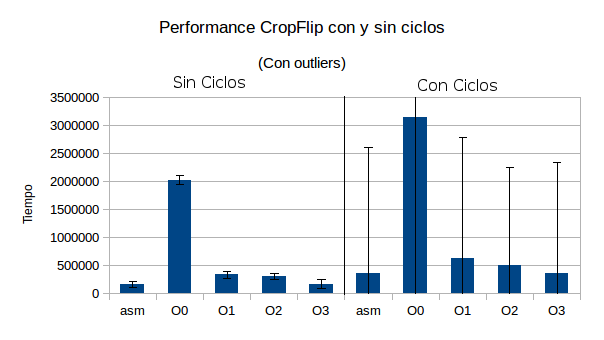
\includegraphics[scale=0.66]{Graficos1.4/1.3/perConOut.png}

Vemos que con loops, el desvío estandar se vuelve incontrolable, a tal punto que sería imposible sacar ninguna conclución de los datos obtenidos. Ahora para intentar mejorar un poco las mediciones, quitamos los $200$ valores mas grandes y los $200$ valores mas chicos (estos van a ser nuestros outliers).

Volvemos a graficar:

  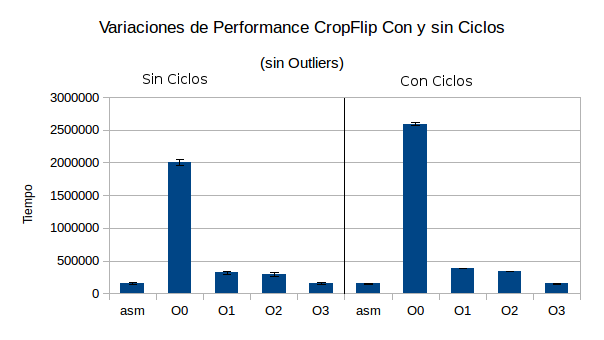
\includegraphics[scale=0.66]{Graficos1.4/1.3/perSinOut.png}

De esta manera logramos obtener valores mucho mas razonables para el desvío estandar.

De este ultimo grafico ademas podemos observar que los loops afectan de manera diferente a los algoritmos, el codigo de C sin optimizar aumenta su tiempo de ejecución en un 25 \%, mientras que el codigo de assambler no varía en lo mas minimo.

Finalmente se determina que para cada experimento en el presente informe, se tomaran 1000 mediciones sin loops corriendo y quitando los outliers antes mencionados.

\newpage

\section{Experimentación}

\subsection{Desensamblado de código C y Optimización}

Comenzamos analizando el código de Cropflip realizado en C.

Este básicamente solo mueve datos de un lugar de la RAM a otros, sin afectar mayormente la imagen.

Realizamos un objdump para ver el código que genera el compilador gcc. Al desensamblar el código pudimos observar, primero que nada, que C guarda todos los parámetros en la pila y además está escribiendo en memoria todas las variables locales utilizadas, lo cual es innecesario ya que pueden ser almacenadas en registros.

También puede observarse que C utiliza saltos incondicionales, lo que puede sugerir que intenta sacar provecho al sistema de predicción de saltos.

Ademas C genera, luego de la función, un montón de secciones que comienzan con debug_xxx. Estas secciones sirven para ser interpretadas por GDB u otros debuggers.

Como ya dijimos, el código podría optimizarse para no realizar tantos accesos a memoria innecesarios guardando variables locales por ejemplo en registros, lo cual disminuiría el tiempo de ejecución.

Luego de esto, procedemos a compilar el código utilizando el flag -O1, y nuevamente realizamos un objdump para ver el código desensamblado. Se observa que ahora el mismo solo realiza los accesos a memoria mínimos indispensables, utilizando los registros para guardar los datos. Además el código es más compacto, y resulta mas claro de leer. Asimismo precalcula los valores que serán utilizados muchas veces, lo que aumenta la performance, principalmente en casos de instancias grandes.

Los otros flags de optimización son -O2, -O3, -Og, -Os, -Ofast. También podemos encontrar los flags -msse, -msse2, -msse3, -mmmx, -m3dnow, pero al intentar compilar con varios de ellos vimos que gcc no utilizó instrucciones SIMD.

Tres nombres de optimizaciones son: -foptimize-sibling-calls, -finline-small-functions, -fmerge-constants.

El flag -foptimize-sibling-calls, sirve para optimizar las funciones con recurcion a la cola.

-finline-small-functions integra funciones a las funciones que las llaman cuando el cuerpo de la función es menor que la cantidad de instrucciones necesarias para llararla, resultando en un codigo de menor tamaño.

-fmerge-constants intenta mergear constantes identicas entre las distintas unidades de compilación.

\newpage

\section{Cropflip}

\subsection{Diferencias de performance en Cropflip}
En el siguiente experimento se medirán las performances tanto de nuestro algoritmo en assembler, implementado para sacar provecho de las instrucciones SSE de Intel, como una versión alternativa hecha en C con diversos grados de optimización a cargo del compilador.

El algoritmo de Cropflip en assembler es muy sencillo. Simplemente movemos 128-bits de la imagen a un xmm y de allí al destino, que previamente ha sido seteado para colocar los bits en el lugar correcto. De esta manera, podremos mover de una sola vez, 16 bytes, lo que corresponde a 4 píxels de la imagen.

Dado que la cantidad de columnas es siempre múltiplo de 4, o sea, siempre tenemos 4 bytes para tomar, no es necesario chequear otros casos borde.

Lo obtenido en los tests puede verse en el siguiente gráfico:

\begin{figure}[h!]
  \begin{center}
	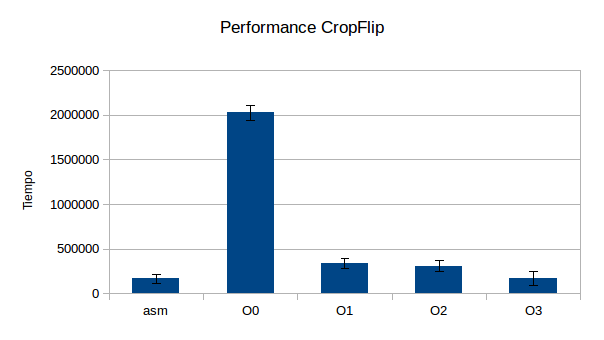
\includegraphics[scale=0.66]{Graficos1.4/crop/per.jpg}
	\label{nombreparareferenciar5}
  \end{center}
\end{figure}

\subsubsection{Resultados}

Se percibe en el gráfico que la version SIMD del algoritmo de cropflip  y la version C con mayor grado de optimización son muy parecidas en promedio, aunque la varianza del codigo C es levemente mayor la del primero. Por otro lado, el programa SIMD tiene una mayor performance a las optimizaciones O1 y O2, y la comparación con O0 muestra que en promedio, es más de 8 veces más rápido.

\subsubsection{Conclusiones}
Una de las razones por las que el codigo optimizado a nivel 3 puede obtener tan buenos resultados como los de SIMD, es que al optimizar con este nivel se activa un flag conocido como "-fipa-cp-clone" que permite hacer algo llamado interprocedural constant propagation, que segun entendemos intenta paralelizar el codigo, o alguna otra optimización del codigo que lo hace extremadamente performante incluso sin utilizar SIMD. Aun asi, prestandole mas atención al desvio estandar, pareciera que este codigo tiene una mayor variabilidad que nuestro codigo en asambler, asi que aun asi, nuestro codigo pareciera tener alguna ventaja sobre el creado en C.

\newpage

\subsection{cpu vs. bus de memoria en Cropflip}

Para este experimento lo que hicimos fue agregar instrucciones aritméticas por un lado y instrucciones de lectura-escritura por otro para ver como influía esto en el tiempo de ejecución de nuestro codigo en assambler.

Para eso agregamos $4$, $8$ y $16$ instrucciones de lectura-escritura por un lado y $4$, $8$ y $16$ instrucciones aritmeticas entre registros en el loop principal del codigo assambler y comparamos las performance entre sí y con la versión original.

Lo que obtuvimos puede verse en el siguiente grafico:

\begin{figure}[h!]
  \begin{center}
  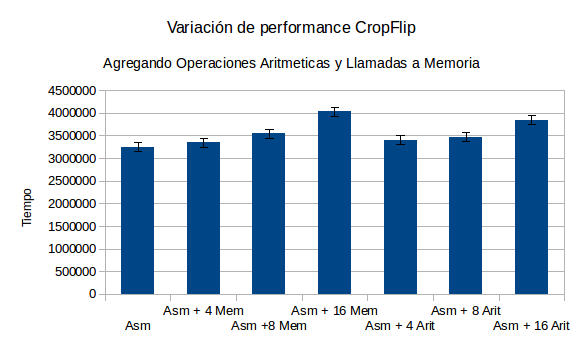
\includegraphics[scale=0.66]{Graficos1.5/crop/per.png}
  \label{nombreparareferenciar1}
  \end{center}
\end{figure}

\subsubsection{Resultados}
Lo que vemos en este grafico es que, si bien al agregar tanto operaciones aritmeticas como operaciones de memoria, el tiempo aumenta, al comparar la misma cantidad de operaciones aritmeticas contra operaciones de lectura-escritura(Mas notoriamente si se comparan entre si el codigo con $16$ operaciones aritmeticas contra el codigo con $16$ operaciones de lectura escritura), las segundas producen un mayor incremento en el tiempo de ejecución del algoritmo.

\subsubsection{Conclusiones}

Lo obtenido en los resultados era de esperar ya que es sabido que el cuello de botella del modelo Bon-Newman y en las arquitecturas modernas, ocurre con los accesos a memoria. En otras palabras, de aquí se puede comprobar de manera empirica que para el procesador es mas costoso acceder a memoria que realizar operaciones logicas, de ahí la diferencia de tiempos que puede observarse. 

\newpage
\section{Sierpinski}

\subsection{Idea general del algoritmo}

Comenzaremos esta sección describiendo la idea tras el algoritmo de Sierpinski. En este caso, el algoritmo ya es un poco más complejo. Necesitamos calcular para cada píxel un coeficiente diferente, que dependerá de la posición $(i,j)$ de cada píxel.
\\
Luego para poder paralelizar de alguna manera el algoritmo en C y sacar provecho a los registros xmm, es necesario calcular 4 coeficientes a la vez y multiplicárselos a sus respectivos píxels.
\\
Luego la idea del algoritmo será algo así:

Al comenzar el ciclo, leemos 4 píxels y los guardamos en un registro xmm. Luego, calculamos el coeficiente para cada píxel de forma paralela como se muestra en el dibujo.


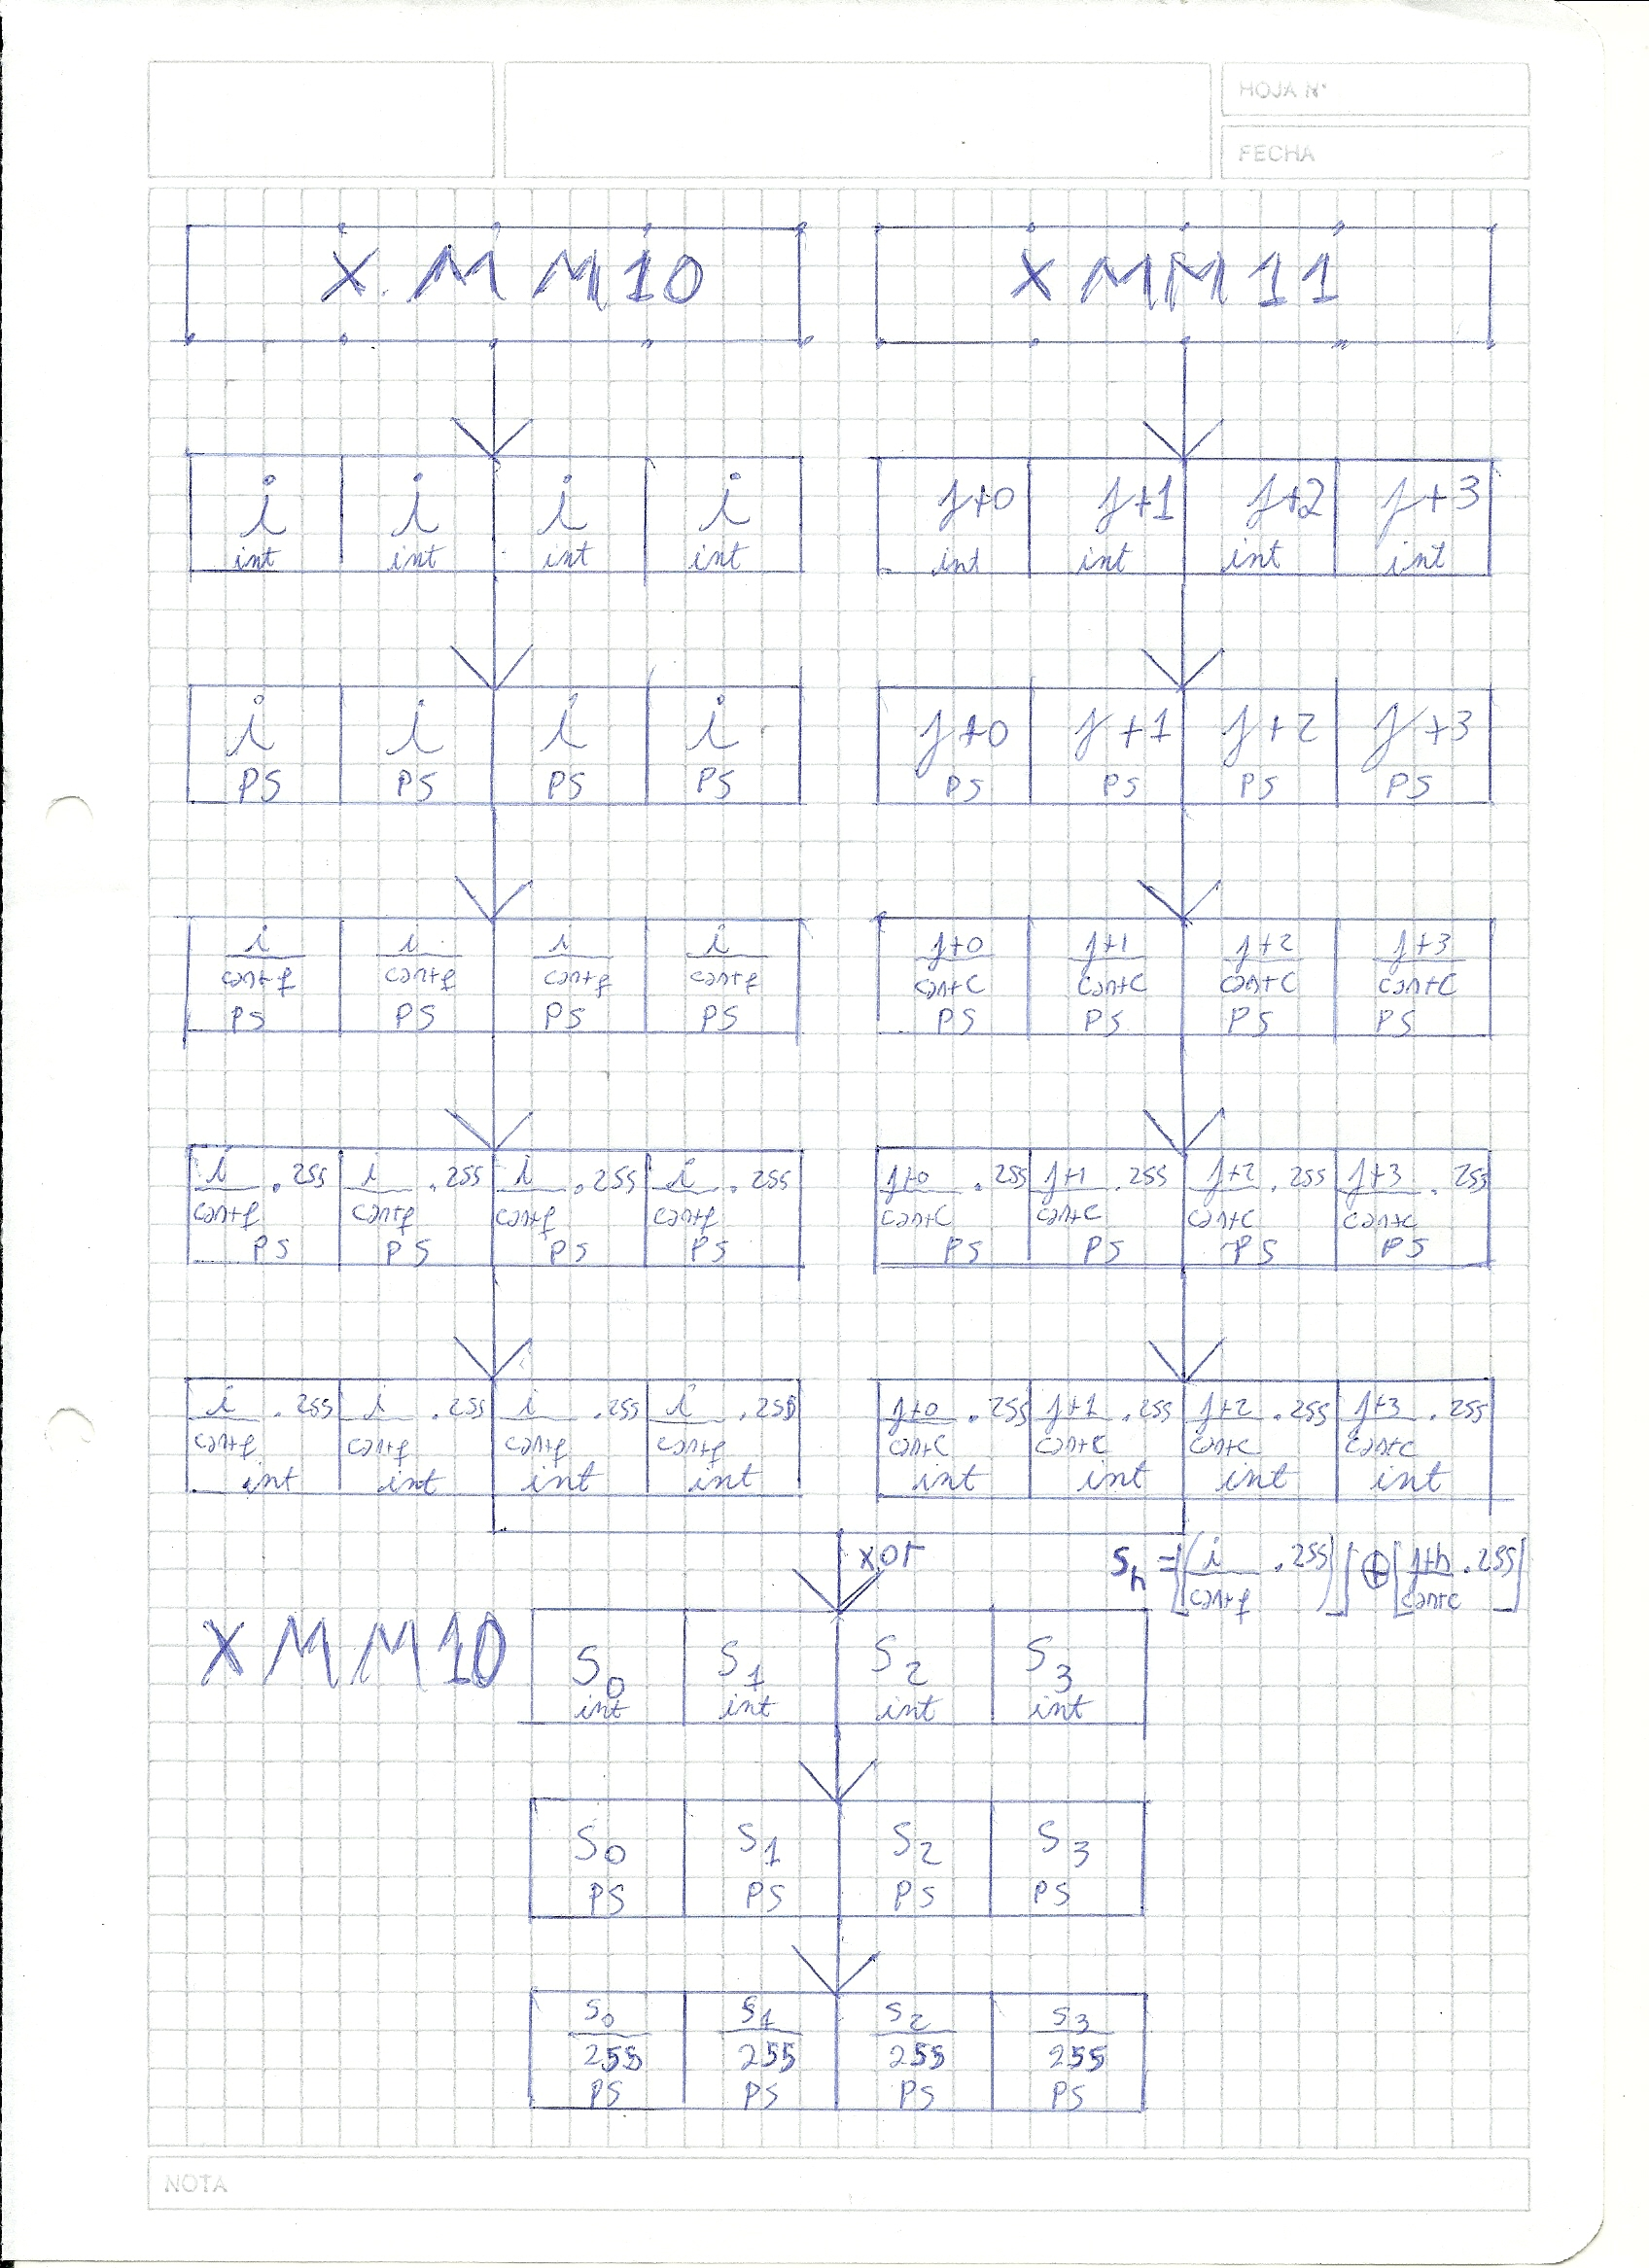
\includegraphics[scale=0.23]{Dibujos/S1.jpg}


Una vez obtenidos los coeficientes, sólo nos resta multiplicar a cada uno por el píxel correspondiente. Como debemos multiplicar dicho coeficiente por cada byte de cada píxel, primero deberemos desempaquetar los datos de tal manera que nos queden 4 registros xmm, uno para cada píxel, que cada uno contenga todos los bytes del píxel asociado en el orden original. A continuación, nos toca convertir todo a punto flotante para poder realizar la multiplicación. Además necesitaremos brodcastear el coeficiente de cada píxel en un registro xmm para así efectivamente multiplicarlo por cada componente del píxel.[ACÁ NO SÉ SI IRÍA DIBUJO DE CÓMO SE HARÍA ESTA MULTIPLICACIÓN, Y EN ESE CASO NO SÉ SI ESTARÍA DE MÁS DEJAR LA ANTERIOR EXPLICACIÓN] Después de terminar con las multiplicaciones, convertimos a entero nuevamente y empaquetamos todo para finalmente moverlo al destino.

\begin{itemize}
\item En la sección data guardamos una constante con el valor 255 brodcasteado en punto flotante.
\item Previo al ciclo, guardamos este valor en un registro.
\item Ya dentro del ciclo, leemos 4 píxels y los guardamos en un xmm.
\item A continuación calculamos de manera paralela para cada píxel el coeficiente correspondiente.
\item Primero, realizamos la división de i por la cantidad de filas y j por la cantidad de columnas, para la cual previamente pasamos de entero a punto flotante.
\item Multiplicamos ambos valores por 255 y luego convertimos a entero con truncamiento.
\item Realizamos un xor entre ambos y despues, volvemos a convertir a punto flotante para dividir por 255.
\item Ya con los coeficientes calculados, solo nos resta multiplicar cada uno por el píxel correspondiente.
\item Para ello desempaquetamos cada byte de cada píxel leido a word, y luego de word a dword, para así convertirlo a punto flotante.
\item Una vez hecha la conversión, brodcasteamos cada coeficiente para poder multiplicarlo por el píxel correspondiente.
\item Luego convertimos a entero nuevamente y empaquetamos todo de dword a word y de word a byte.
\item Y finalmente movemos los píxels procesados al destino.
\end{itemize}

\subsection{Diferencias de performance en Sierpinski}

Los resultados comparativos de performance para este algoritmo comparado con uno desarrollado en C fueron los siguientes:

\newpage

\begin{figure}[h!]
  \begin{center}
  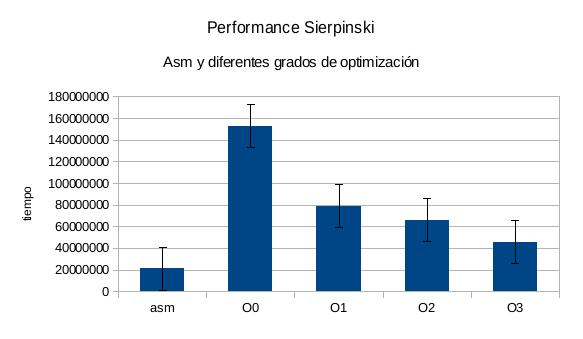
\includegraphics[scale=0.66]{Graficos1.4/sie/per.jpg}
  \label{nombreparareferenciar7}
  \end{center}
\end{figure}

\subsubsection{Resultados}
Puede verse que en este caso, nuestro codigo en assambler, que toma y calcula de a 4 píxels utilizando instrucciones SIMD tiene, en promedio, una mejor performance que los demás. En el grafico puede notarse que este codigo es aproximadamente dos veces más rápido que la versión de C con O3, más de tres veces más rápido que O2 y O1 y más de 7 veces más veloz que O0, todo esto en promedio. El desvio estandar en este caso es tan pequeño que casi no puede verse en el grafico.
\subsubsection{Conclusiones}

De lo que podemos observar, concluímos que en este caso, paralelizar los datos y operar sobre ellos resulta en un incremento de la performance incluso superior al codigo en C con mayor grado de optimización-

\newpage
\subsection{CPU vs. Bus de memoria en Sierpinski}

Realizamos el mismo experimento que hicimos para cropflip, es decir, agregamos instrucciones aritmeticas y de lectura escritura al codigo assambler para medir su desempeño.

Tomando el primedio y graficando los valores obtenidos:

\begin{figure}[h!]
  \begin{center}
  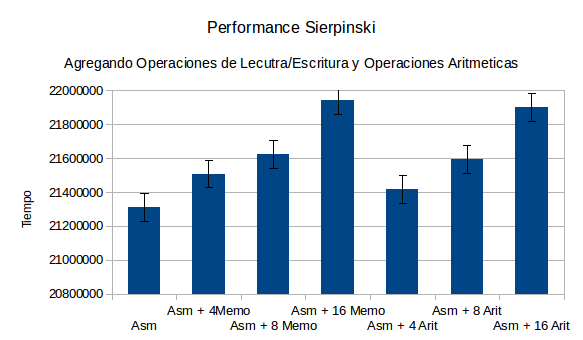
\includegraphics[scale=0.66]{Graficos1.5/sie/per.png}
  \label{nombreparareferenciar1}
  \end{center}
\end{figure}

\subsubsection{Resultados}
Nuevamente, como es de esperar al agregar operaciones, tanto aritmeticas como de lectura-escritura, el tiempo de ejecución aumenta. Tambien, como en el caso anterior, al comparar entre agregar un numero de operaciones aritmeticas y agregar el mismo numero de operaciones de lectura-escritura, las operaciones de lectura escritura, son mas caras para el procesador.

\subsubsection{Conclusiones}

Nuevamente podemos llegar a la misma conclución que antes, el cuello de botella se encuentra en el tiempo que el procesador tarda en buscar datos a memoria. Incluso implementando tecnicas abanzadas como caché y ejecución fuera de orden, puede notarse la diferencia. 

Tal vez en este caso la diferencia es menos marcada porque ya se le estaba dando un uso exaustivo a la ALU y agregar mas operaciones aritmeticas resulta mas costoso aquí que en el caso del cropflip, donde la ALU no era mayormente utilizada.

\newpage
\section{Bandas}
\subsection{Idea general del algoritmo}
Para el algoritmo de bandas se nos presenta otro desafío: debemos tomar los tres colores de la imagen $(r,g,b)$, sumarlos, y luego comparar cada uno de ellos para ver si se encuentra en un rango determinado.
\\
Para resolver la primera problemática usaremos las instrucciones $phaddw$, que nos permitirá a través de una suma horizontal, sumar los valores r,g,b de manera cómoda solamente utilizando dos registros.
\\
El segundo problema será comparar estos valores obtenidos en la suma de una manera eficiente. Querríamos compararlos todos a la vez y a partir de esas comparaciones determinar que valores deberá ir en cada píxel. Esta se resolverá utilizando broadcasting. El algoritmo irá comparando en cada paso contra un valor y en caso de cumplirse una condición, restará donde corresponda.

Como primer paso, leemos los 4 píxels y los guardamos en un xmm. Luego, desempaquetamos los datos de byte a word para poder realizar la suma de las componentes de cada píxel sin salirnos de la representación. La suma se hace a través de dos instrucciones de suma horizontal, como mencionamos anteriormente, de tal manera que nos quedan los $b$ de cada píxel en las cuatro words de la parte baja de un xmm. A continuación realizamos unas comparaciones utilizando máscaras predefinidas para determinar el valor que tendrá cada píxel en cada una de sus componentes. Después de realizadas estas comparaciones, nos queda en las word de la parte baja de un xmm los 4 valores que se asignarán a cada componente de cada píxel. Luego, empaquetamos estos valores pasandolos de word a byte y aplicamos un shuffle que los deja en el los lugares que corresponden para finalmente copiarlos al destino. 

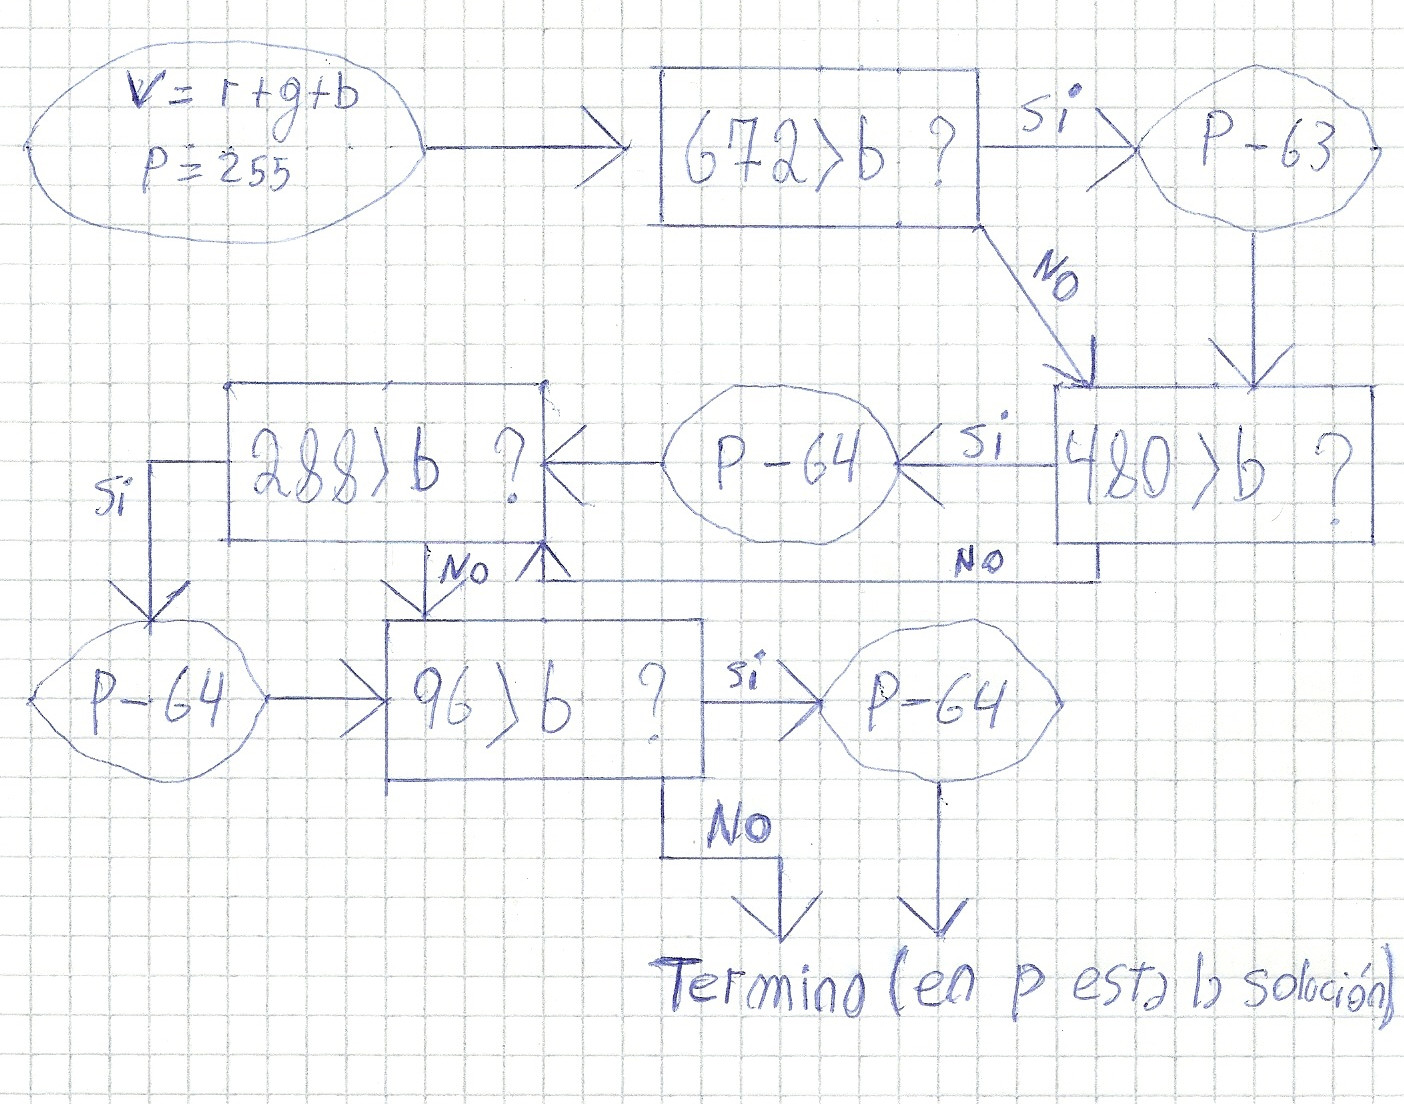
\includegraphics[scale=0.66]{Dibujos/B1.jpg}


\begin{itemize}
\item  En la sección data tenemos mascaras y constantes brodcasteadas que utilizaremos para hacer las comparaciones.
\item  Ademas en esta sección tenemos una doble qword la cual usaremos para el shuffle final.
\item  Previo al ciclo donde procesamos los píxels, movemos estos datos a registros xmm.
\item  Ya una vez dentro del ciclo, leemos 4 píxels y los guardamos en un xmm.
\item  Desempaquetamos los bytes a word para poder hacer la suma de las componentes de cada píxel sin irnos de la representación.
\item  Hacemos dos sumas horizontales para obtener los cuatro valores  de b.
\item  Luego utilizamos las mascaras para comparar en paralelo cada píxel con el b correspondiente y asignando el valor de rgb segun corresponda.
\item  Nos queda en cada word de la parte baja de un xmm, los 4 valores que se asignaran a cada rgb de cada píxel.
\item  Finalmente, empaquetamos estos valores para volver a byte y los shuffleamos para dejarlos en los lugares correspondiente y lo asignamos en el destino.
\end{itemize}

\subsection{Diferencias de performance en Bandas}

Los resultados de los tiempos comparativos son los siguientes:

\newpage

\begin{figure}[h!]
  \begin{center}
  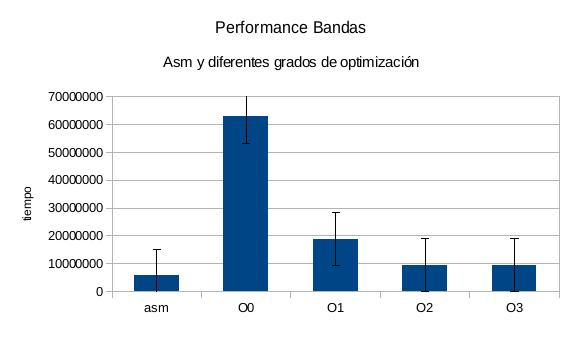
\includegraphics[scale=0.66]{Graficos1.4/ban/per.jpg}
  \label{nombreparareferenciar9}
  \end{center}
\end{figure}

\subsubsection{Resultados}
Otra vez puede observarse que en promedio el algoritmo en assambler que se vale de instrucciones vectoriales es superior a su contraparte en C. Incluso con el mayor grado de optimización nuestro algoritmo logra ser casi un 50 \% mejor que el codigo en C con mayor grado de optimización. Para esta escala el desvío estandar no es apreciable ya que es un orden de magnitud menor.

\subsubsection{Conclusiones}

Nuevamente podemos concluir que resulta ventajoso utilizar instrucciones vectoriales para realizar calculos paralelizados sobre un gran volumen de datos.

\newpage
\subsection{Saltos condicionales}

En este experimento veremos como afectan los saltos condicionales a la performance del codigo C compilado con -O1. Para ello lo que haremos es quitar los IFs del codigo dejando solo una banda, luego medir la performance y compararla con la version con saltos.

\begin{figure}[h!]
  \begin{center}
  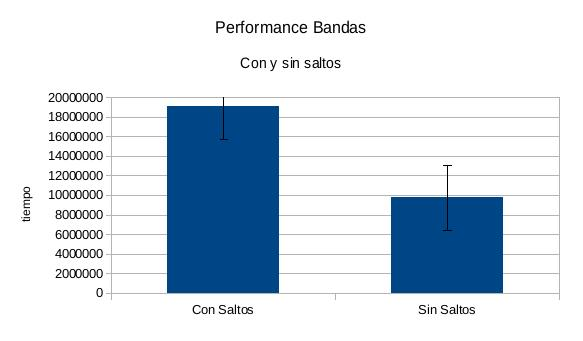
\includegraphics[scale=0.66]{Graficos3.1/per.jpg}
  \label{nombreparareferenciar1}
  \end{center}
\end{figure}

\subsubsection{Resultados}
En el grafico puede observarse una gran diferencia entre el codigo que tiene saltos condicionales y el codigo que no los tiene. La varianza tambien es levemente diferente, $301534$ del codigo con saltos a $109026$ sin los mismos.

\subsubsection{Conclusiones}

La variación de tiempos ocurre posiblemente debido a que en el caso del codigo con saltos, el procesador intentará predecir el salto, conocido como branch prediction, tomado todas las posibles ramas de la ejecución. Esto sin duda causará que el procesador este mas ocupado realizando calculos en todas las ramas y aumente el tiempo de ejecuión. Esto también explicaría el aumento en la variabilidad, ya que el el CPU se vuelve menos predecible.

\newpage
\subsection{Motion Blur}
\subsection{Idea general del algoritmo}
La idea de este algoritmo es, por cada píxel del destino se deben tomar 5 píxels de la entrada, se multiplica cada uno de los colores por $0.2$ y luego se los suma. Lo que realmente haremos en el algoritmo será primero hacer la suma y luego multiplicar por $0.2$ ya que esto requiere menos registros XMM.
\\
Para ello debemos tener cuidado de tomar correctamente los casos borde y no aplicar motion blur donde no corresponde.
\\
Una idea general de cómo funciona el algoritmo en assembler es la siguiente:

Al comenzar el ciclo, esta vez no sólo leeremos 4 píxels, sino que también leeremos píxeles de las filas vecinas ya que para procesar un píxel $(i,j)$ necesitaremos además los 4 píxels de las filas $i-2$, $i-1$, $i+1$ e $i+2$ en las columnas $j-2$, $j-1$, $j$, $j+1$ y $j+2$, respectivamente. Luego, desempaquetamos todo a word para realizar la sumas sin irnos de la representación. Cuando ya hemos sumado lo que necesitamos, desempaquetamos nuevamente pero ahora a dword para poder convertir a punto flotante y así luego multiplicar por $0.2$. Una vez realizada la multiplicación, convertimos a entero nuevamente y empaquetamos todo de dword a word, y de word a byte. Finalmente, copiamos los 4 píxels procesados al destino. Además de todo esto, cada vez que terminamos de recorrer una fila, ponemos en negro los siguientes 4 píxels, y las dos primeras y últimas filas las ponemos en negro aparte, fuera del ciclo.

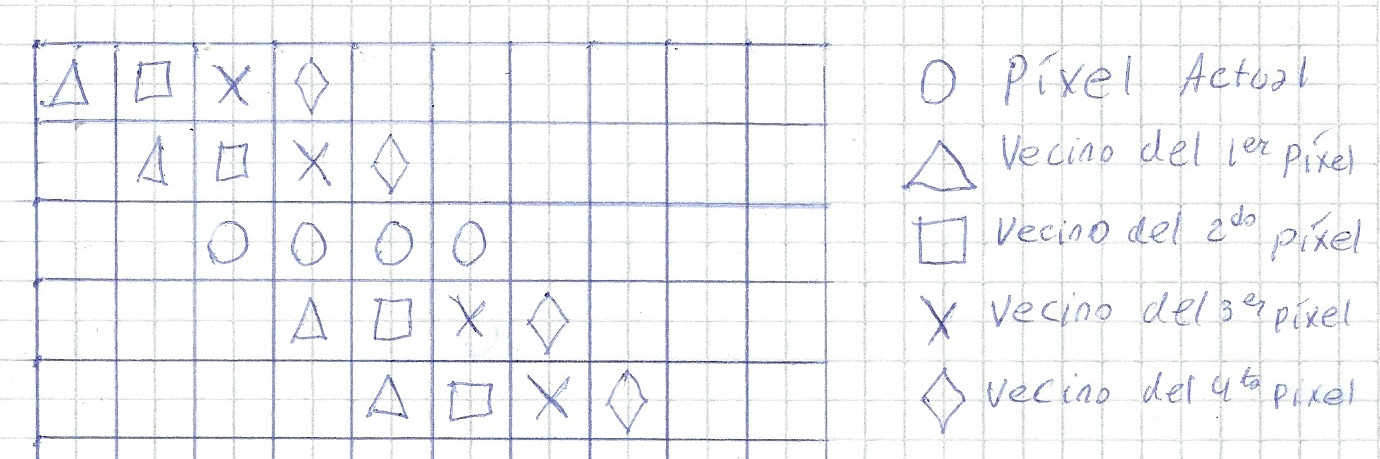
\includegraphics[scale=0.66]{Dibujos/MB1.jpg}

\begin{itemize}
\item  Tenemos, en la sección datos, el valor $0.2$ brodcasteado que utilizaremos para realizar la multiplicación.
\item  Previo al procesamiento de datos, guardamos en un xmm este valor.
\item  Dentro del ciclo, para procesar el píxel (i,j) tomamos los 4 píxels de las filas $i-2$, $i-1$, $i$, $i+1$ e $i+2$ a partir de la columna $j-2$, $j-1$, $j$, $j+1$ y $j+2$, respectivamente, y almacenamos todo en registros.
\item  Desempaquetamos todo a word para poder hacer la suma sin desbordar.
\item  Luego de realizar las sumas, desempaquetamos a dwords para así poder convertir a punto flotante.
\item  Con la conversión ya hecha, podemos multiplicar cada valor por $0.2$.
\item  Convertimos a entero nuevamente y empaquetamos de dword a word y de word a byte.
\item  Finalmente, copiamos los 4 píxels resultantes al destino. 
\item  Cada vez que termino de recorrer una fila, pongo en negro los siguientes 4 píxels, y las dos primeras y últimas filas las pongo en negro aparte, fuera del ciclo.
\end{itemize}

\subsection{Diferencias de performance en Motion Blur}

Al realizar el testing se obtuvieron los siguientes resultados:

\newpage

\begin{figure}[h!]
  \begin{center}
  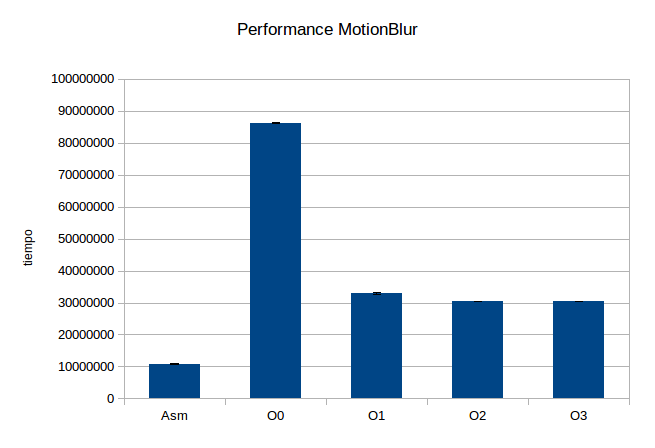
\includegraphics[scale=0.66]{Graficos1.4/mbl/per.jpg}
  \label{nombreparareferenciar11}
  \end{center}
\end{figure}

\subsubsection{Resultados}
Se aprecia en el gráfico que el código ASM con SIMD tiene un promedio de tiempo de ejecucion aproximadamente tres veces menor a la mayor optimización de C, y varias veces menor que O0. También se observa que O1, como O2 y O3 dan promedios de tiempo muy parecidos. Las varianzas son similares y muy pequeñas.

\subsubsection{Conclusiones}

En este caso podemos concluir nuevamente que la opcion en assambler es mejor que la opción en C que no utiliza operaciones vectoriales, incluso con el mayor grado de optimización.

\newpage
\section{Conclusiones y trabajo futuro}

Como primera conclución de este trabajo practico podemos decir la gran ventaja que reperesenta la utilización de operaciones vectoriales a la hora de realizar operaciones paralelizables sobre un gran volumen de datos. Tambien podemos concluir que esto no resulta de la misma manera en el caso de transferir información de un lugar de la memoria RAM a otro, ahí, la opción de implementar codigo C optimizado es tan buena como la de implementarlo con SIMD, con la ventaja de que en C el codigo es mas facilmente mantenible y claro.

Otras concluciones son, que la comprobación de manera empirica que el acceso a RAM presenta una mayor caída de performance que las operaciones aritmeticas. Y que el brunch prediction tambien representa una mayor caida en la performance, por lo que utilizar otras opciones que no requieran saltos condicionales es una buena opción de mejorar los tiempos de un algoritmo dado.

Como trabajo futuro, una idea interesante a desarollar, podría ser construir o plantear un compilador de C que tome la mejor parte de los compiladores actuales, esto es, las diversas optimizaciones que realiza, y las integre con SIMD. De esta manera se podría en teoría obtenerse mejores resultados que los aquí mostrados.

\end{document}

